% **************************************************************************************************************
% A Classic Thesis Style
% An Homage to The Elements of Typographic Style
%
% Copyright (C) 2015 André Miede http://www.miede.de
%
% If you like the style then I would appreciate a postcard. My address 
% can be found in the file ClassicThesis.pdf. A collection of the 
% postcards I received so far is available online at 
% http://postcards.miede.de
%
% License:
% This program is free software; you can redistribute it and/or modify
% it under the terms of the GNU General Public License as published by
% the Free Software Foundation; either version 2 of the License, or
% (at your option) any later version.
%
% This program is distributed in the hope that it will be useful,
% but WITHOUT ANY WARRANTY; without even the implied warranty of
% MERCHANTABILITY or FITNESS FOR A PARTICULAR PURPOSE.  See the
% GNU General Public License for more details.
%
% You should have received a copy of the GNU General Public License
% along with this program; see the file COPYING.  If not, write to
% the Free Software Foundation, Inc., 59 Temple Place - Suite 330,
% Boston, MA 02111-1307, USA.
%
% **************************************************************************************************************
\RequirePackage{fix-cm} % fix some latex issues see: http://texdoc.net/texmf-dist/doc/latex/base/fixltx2e.pdf
\documentclass[ twoside,openright,titlepage,numbers=noenddot,headinclude,%1headlines,% letterpaper a4paper
                footinclude=true,cleardoublepage=empty,abstractoff, % <--- obsolete, remove (todo)
                BCOR=5mm,paper=a4,fontsize=11pt,%11pt,a4paper,%
                ngerman,american,%
                ]{scrreprt}

% ****************************************************************************************************
% Set the encoding of your files. UTF-8 is the only sensible encoding nowadays. If you can't read
% äöüßáéçèê∂åëæƒÏ€ then change the encoding setting in your editor, not the line below. If your editor
% does not support utf8 use another editor!
% ****************************************************************************************************
\PassOptionsToPackage{utf8}{inputenc}
	\usepackage{inputenc}
	
\usepackage{etoolbox}

% ****************************************************************************************************
% Insert the information about your thesis here
% ****************************************************************************************************
\newcommand{\myTitle}{AnSiAn - Android Signal Analyzer\xspace}
\newcommand{\myDegree}{SEEMOO Secure Networking Lab\xspace}
\newcommand{\myName}{Dennis Mantz and Max Engelhardt\xspace}
\newcommand{\myProf}{Prof. Dr.-Ing. Matthias Hollick\xspace}
%\newcommand{\myOtherProf}{Second advisor\xspace}
\newcommand{\mySupervisor}{Jiska Classen}
\newcommand{\myFaculty}{Department of Computer Science\xspace}
\newcommand{\myDepartment}{Secure Mobile Networking Lab\xspace}
\newcommand{\myUni}{\protect{Technische Universität Darmstadt}\xspace}
\newcommand{\myLocation}{Darmstadt\xspace}
\newcommand{\myTime}{\formatdate{28}{04}{2016}\xspace}
\newcommand{\myVersion}{0.1\xspace}

% Choose if you want the standard template with enough space for margin notes or the tempate with small margins
\newtoggle{adrianstyle}
%\toggletrue{adrianstyle} % uncomment this line to have smaller margins
\togglefalse{adrianstyle} % uncomment this line for the standard seemoo template

%********************************************************************
% Note: Make all your adjustments in here
%*******************************************************
% ****************************************************************************************************
% classicthesis-config.tex 
% formerly known as loadpackages.sty, classicthesis-ldpkg.sty, and classicthesis-preamble.sty 
% Use it at the beginning of your ClassicThesis.tex, or as a LaTeX Preamble 
% in your ClassicThesis.{tex,lyx} with % ****************************************************************************************************
% classicthesis-config.tex 
% formerly known as loadpackages.sty, classicthesis-ldpkg.sty, and classicthesis-preamble.sty 
% Use it at the beginning of your ClassicThesis.tex, or as a LaTeX Preamble 
% in your ClassicThesis.{tex,lyx} with % ****************************************************************************************************
% classicthesis-config.tex 
% formerly known as loadpackages.sty, classicthesis-ldpkg.sty, and classicthesis-preamble.sty 
% Use it at the beginning of your ClassicThesis.tex, or as a LaTeX Preamble 
% in your ClassicThesis.{tex,lyx} with \input{classicthesis-config}
% ****************************************************************************************************  
% If you like the classicthesis, then I would appreciate a postcard. 
% My address can be found in the file ClassicThesis.pdf. A collection 
% of the postcards I received so far is available online at 
% http://postcards.miede.de
% ****************************************************************************************************

% ****************************************************************************************************
% 1. Configure classicthesis for your needs here, e.g., remove "drafting" below 
% in order to deactivate the time-stamp on the pages
% ****************************************************************************************************
\PassOptionsToPackage{eulerchapternumbers,listings,%
                 %drafting,%
				 pdfspacing,%floatperchapter,%linedheaders,%
				 subfig,beramono,eulermath,parts,dottedtoc,%
				 \iftoggle{adrianstyle}{adrianstyle}{}, % Use this option to increase the text width
				 }{classicthesis}								
% ********************************************************************
% Available options for classicthesis.sty 
% (see ClassicThesis.pdf for more information):
% drafting
% parts nochapters linedheaders
% eulerchapternumbers beramono eulermath pdfspacing minionprospacing
% tocaligned dottedtoc manychapters
% listings floatperchapter subfig
% ********************************************************************


% ****************************************************************************************************
% 2. Loading some handy packages
% ****************************************************************************************************
%\PassOptionsToPackage{spanish,es-lcroman}{babel}

% ********************************************************************
% Setup, finetuning, and useful commands
% ********************************************************************
\newcounter{dummy} % necessary for correct hyperlinks (to index, bib, etc.)
\newlength{\abcd} % for ab..z string length calculation
% ****************************************************************************************************


% ****************************************************************************************************
% 3. Loading some handy packages
% ****************************************************************************************************
% ******************************************************************** 
% Packages with options that might require adjustments
% ******************************************************************** 
%\PassOptionsToPackage{ngerman,american}{babel}   % change this to your language(s)
% Spanish languages need extra options in order to work with this template
%\PassOptionsToPackage{spanish,es-lcroman}{babel}
	\usepackage{babel}                  

\usepackage{csquotes}
\PassOptionsToPackage{%
    %backend=biber, %instead of bibtex
	backend=bibtex8,bibencoding=ascii,%
	language=auto,%
	style=numeric-comp,%
    %style=authoryear-comp, % Author 1999, 2010
    %bibstyle=authoryear,dashed=false, % dashed: substitute rep. author with ---
    sorting=nyt, % name, year, title
    maxbibnames=10, % default: 3, et al.
    %backref=true,%
    natbib=true % natbib compatibility mode (\citep and \citet still work)
}{biblatex}
    \usepackage{biblatex}

\PassOptionsToPackage{fleqn}{amsmath}       % math environments and more by the AMS 
    \usepackage{amsmath}

% ******************************************************************** 
% General useful packages
% ******************************************************************** 
\PassOptionsToPackage{T1}{fontenc} % T2A for cyrillics
    \usepackage{fontenc}     
\usepackage{textcomp} % fix warning with missing font shapes
\usepackage{scrhack} % fix warnings when using KOMA with listings package          
\usepackage{xspace} % to get the spacing after macros right  
\usepackage{mparhack} % get marginpar right
\usepackage{fixltx2e} % fixes some LaTeX stuff --> since 2015 in the LaTeX kernel (see below)
%\usepackage[latest]{latexrelease} % will be used once available in more distributions (ISSUE #107)
\usepackage[nopostdot,acronym,shortcuts,nonumberlist]{glossaries}
\makeglossaries
\renewcommand*{\glossarysection}[2][]{}
\input{acronyms.tex}
% ****************************************************************************************************


% ****************************************************************************************************
% 4. Setup floats: tables, (sub)figures, and captions
% ****************************************************************************************************
\usepackage{tabularx} % better tables
    \setlength{\extrarowheight}{3pt} % increase table row height
\newcommand{\tableheadline}[1]{\multicolumn{1}{c}{\spacedlowsmallcaps{#1}}}
\newcommand{\myfloatalign}{\centering} % to be used with each float for alignment
\usepackage{caption}
% Thanks to cgnieder and Claus Lahiri
% http://tex.stackexchange.com/questions/69349/spacedlowsmallcaps-in-caption-label
% [REMOVED DUE TO OTHER PROBLEMS, SEE ISSUE #82]    
%\DeclareCaptionLabelFormat{smallcaps}{\bothIfFirst{#1}{~}\MakeTextLowercase{\textsc{#2}}}
%\captionsetup{font=small,labelformat=smallcaps} % format=hang,
\captionsetup{font=small} % format=hang,
\usepackage{subfig}  
% ****************************************************************************************************


% ****************************************************************************************************
% 5. Setup code listings
% ****************************************************************************************************
\usepackage{listings} 
%\lstset{emph={trueIndex,root},emphstyle=\color{BlueViolet}}%\underbar} % for special keywords
\lstset{language=[LaTeX]Tex,%C++,
    morekeywords={PassOptionsToPackage,selectlanguage},
    keywordstyle=\color{RoyalBlue},%\bfseries,
    basicstyle=\small\ttfamily,
    %identifierstyle=\color{NavyBlue},
    commentstyle=\color{Green}\ttfamily,
    stringstyle=\rmfamily,
    numbers=none,%left,%
    numberstyle=\scriptsize,%\tiny
    stepnumber=5,
    numbersep=8pt,
    showstringspaces=false,
    breaklines=true,
    %frameround=ftff,
    %frame=single,
    belowcaptionskip=.75\baselineskip
    %frame=L
} 
% ****************************************************************************************************    		   


% ****************************************************************************************************
% 6. PDFLaTeX, hyperreferences and citation backreferences
% ****************************************************************************************************
% ********************************************************************
% Using PDFLaTeX
% ********************************************************************
\PassOptionsToPackage{pdftex,hyperfootnotes=false,pdfpagelabels}{hyperref}
    \usepackage{hyperref}  % backref linktocpage pagebackref
\pdfcompresslevel=9
\pdfadjustspacing=1 
\PassOptionsToPackage{pdftex}{graphicx}
    \usepackage{graphicx} 
 

% ********************************************************************
% Hyperreferences
% ********************************************************************
\hypersetup{%
    %draft,	% = no hyperlinking at all (useful in b/w printouts)
    %colorlinks=true, linktocpage=true, pdfstartpage=3, pdfstartview=FitV,%
    % uncomment the following line if you want to have black links (e.g., for printing)
    colorlinks=false, linktocpage=false, pdfborder={0 0 0}, pdfstartpage=3, pdfstartview=FitV,% 
    breaklinks=true, pdfpagemode=UseNone, pageanchor=true, pdfpagemode=UseOutlines,%
    plainpages=false, bookmarksnumbered, bookmarksopen=true, bookmarksopenlevel=1,%
    hypertexnames=true, pdfhighlight=/O,%nesting=true,%frenchlinks,%
    urlcolor=webbrown, linkcolor=RoyalBlue, citecolor=webgreen, %pagecolor=RoyalBlue,%
    %urlcolor=Black, linkcolor=Black, citecolor=Black, %pagecolor=Black,%
    pdftitle={\myTitle},%
    pdfauthor={\textcopyright\ \myName, \myUni, \myFaculty},%
    pdfsubject={},%
    pdfkeywords={},%
    pdfcreator={pdfLaTeX},%
    pdfproducer={LaTeX with hyperref and classicthesis}%
}

\pdfinfo{
   /CreationDate (D:20130424083342)
   /ModDate (D:20130424083342)
}

% ********************************************************************
% Setup autoreferences
% ********************************************************************
% There are some issues regarding autorefnames
% http://www.ureader.de/msg/136221647.aspx
% http://www.tex.ac.uk/cgi-bin/texfaq2html?label=latexwords
% you have to redefine the makros for the 
% language you use, e.g., american, ngerman
% (as chosen when loading babel/AtBeginDocument)
% ********************************************************************
\makeatletter
\@ifpackageloaded{babel}%
    {%
       \addto\extrasamerican{%
			\renewcommand*{\figureautorefname}{Figure}%
			\renewcommand*{\tableautorefname}{Table}%
			\renewcommand*{\partautorefname}{Part}%
			\renewcommand*{\chapterautorefname}{Chapter}%
			\renewcommand*{\sectionautorefname}{Section}%
			\renewcommand*{\subsectionautorefname}{Section}%
			\renewcommand*{\subsubsectionautorefname}{Section}%     
                }%
       \addto\extrasngerman{% 
			\renewcommand*{\paragraphautorefname}{Absatz}%
			\renewcommand*{\subparagraphautorefname}{Unterabsatz}%
			\renewcommand*{\footnoteautorefname}{Fu\"snote}%
			\renewcommand*{\FancyVerbLineautorefname}{Zeile}%
			\renewcommand*{\theoremautorefname}{Theorem}%
			\renewcommand*{\appendixautorefname}{Anhang}%
			\renewcommand*{\equationautorefname}{Gleichung}%        
			\renewcommand*{\itemautorefname}{Punkt}%
                }%  
            % Fix to getting autorefs for subfigures right (thanks to Belinda Vogt for changing the definition)
            \providecommand{\subfigureautorefname}{\figureautorefname}%             
    }{\relax}
\makeatother


% ****************************************************************************************************
% 7. Last calls before the bar closes
% ****************************************************************************************************
% ********************************************************************
% Development Stuff
% ********************************************************************
\listfiles
%\PassOptionsToPackage{l2tabu,orthodox,abort}{nag}
%   \usepackage{nag}
%\PassOptionsToPackage{warning, all}{onlyamsmath}
%   \usepackage{onlyamsmath}

% ********************************************************************
% Last, but not least...
% ********************************************************************
\usepackage{classicthesis} 
% ****************************************************************************************************


% ****************************************************************************************************
% 8. Further adjustments (experimental)
% ****************************************************************************************************
% ********************************************************************
% Changing the text area
% ********************************************************************
%\linespread{1.05} % a bit more for Palatino
%\areaset[current]{312pt}{761pt} % 686 (factor 2.2) + 33 head + 42 head \the\footskip
%\setlength{\marginparwidth}{7em}%
%\setlength{\marginparsep}{2em}%

% ********************************************************************
% Using different fonts
% ********************************************************************
%\usepackage[oldstylenums]{kpfonts} % oldstyle notextcomp
%\usepackage[osf]{libertine}
%\usepackage[light,condensed,math]{iwona}
%\renewcommand{\sfdefault}{iwona}
%\usepackage{lmodern} % <-- no osf support :-(
%\usepackage{cfr-lm} % 
%\usepackage[urw-garamond]{mathdesign} <-- no osf support :-(
%\usepackage[default,osfigures]{opensans} % scale=0.95 
%\usepackage[sfdefault]{FiraSans}
% ****************************************************************************************************

% ****************************************************************************************************  
% If you like the classicthesis, then I would appreciate a postcard. 
% My address can be found in the file ClassicThesis.pdf. A collection 
% of the postcards I received so far is available online at 
% http://postcards.miede.de
% ****************************************************************************************************

% ****************************************************************************************************
% 1. Configure classicthesis for your needs here, e.g., remove "drafting" below 
% in order to deactivate the time-stamp on the pages
% ****************************************************************************************************
\PassOptionsToPackage{eulerchapternumbers,listings,%
                 %drafting,%
				 pdfspacing,%floatperchapter,%linedheaders,%
				 subfig,beramono,eulermath,parts,dottedtoc,%
				 \iftoggle{adrianstyle}{adrianstyle}{}, % Use this option to increase the text width
				 }{classicthesis}								
% ********************************************************************
% Available options for classicthesis.sty 
% (see ClassicThesis.pdf for more information):
% drafting
% parts nochapters linedheaders
% eulerchapternumbers beramono eulermath pdfspacing minionprospacing
% tocaligned dottedtoc manychapters
% listings floatperchapter subfig
% ********************************************************************


% ****************************************************************************************************
% 2. Loading some handy packages
% ****************************************************************************************************
%\PassOptionsToPackage{spanish,es-lcroman}{babel}

% ********************************************************************
% Setup, finetuning, and useful commands
% ********************************************************************
\newcounter{dummy} % necessary for correct hyperlinks (to index, bib, etc.)
\newlength{\abcd} % for ab..z string length calculation
% ****************************************************************************************************


% ****************************************************************************************************
% 3. Loading some handy packages
% ****************************************************************************************************
% ******************************************************************** 
% Packages with options that might require adjustments
% ******************************************************************** 
%\PassOptionsToPackage{ngerman,american}{babel}   % change this to your language(s)
% Spanish languages need extra options in order to work with this template
%\PassOptionsToPackage{spanish,es-lcroman}{babel}
	\usepackage{babel}                  

\usepackage{csquotes}
\PassOptionsToPackage{%
    %backend=biber, %instead of bibtex
	backend=bibtex8,bibencoding=ascii,%
	language=auto,%
	style=numeric-comp,%
    %style=authoryear-comp, % Author 1999, 2010
    %bibstyle=authoryear,dashed=false, % dashed: substitute rep. author with ---
    sorting=nyt, % name, year, title
    maxbibnames=10, % default: 3, et al.
    %backref=true,%
    natbib=true % natbib compatibility mode (\citep and \citet still work)
}{biblatex}
    \usepackage{biblatex}

\PassOptionsToPackage{fleqn}{amsmath}       % math environments and more by the AMS 
    \usepackage{amsmath}

% ******************************************************************** 
% General useful packages
% ******************************************************************** 
\PassOptionsToPackage{T1}{fontenc} % T2A for cyrillics
    \usepackage{fontenc}     
\usepackage{textcomp} % fix warning with missing font shapes
\usepackage{scrhack} % fix warnings when using KOMA with listings package          
\usepackage{xspace} % to get the spacing after macros right  
\usepackage{mparhack} % get marginpar right
\usepackage{fixltx2e} % fixes some LaTeX stuff --> since 2015 in the LaTeX kernel (see below)
%\usepackage[latest]{latexrelease} % will be used once available in more distributions (ISSUE #107)
\usepackage[nopostdot,acronym,shortcuts,nonumberlist]{glossaries}
\makeglossaries
\renewcommand*{\glossarysection}[2][]{}
\newacronym{USRP}{USRP}{Universal Software Radio Peripheral}
\newacronym{SDR}{SDR}{software-defined radio}
\newacronym{FPGA}{FPGA}{field-programmable gate array}
\newacronym{DAC}{DAC}{digital-to-analog converter}
\newacronym{RF}{RF}{radio frequency}
\newacronym{ADC}{ADC}{analog-to-digital converter}
\newacronym{SNR}{SNR}{signal-to-noise ratio}
\newacronym{AnSiAn}{AnSiAn}{Android Signal Analyzer}
\newacronym{RDS}{RDS}{Radio Data System}
\newacronym{FM}{FM}{frequency modulation}
\newacronym{LSB}{LSB}{lower side band}
\newacronym{USB}{USB}{upper side band}

% ****************************************************************************************************


% ****************************************************************************************************
% 4. Setup floats: tables, (sub)figures, and captions
% ****************************************************************************************************
\usepackage{tabularx} % better tables
    \setlength{\extrarowheight}{3pt} % increase table row height
\newcommand{\tableheadline}[1]{\multicolumn{1}{c}{\spacedlowsmallcaps{#1}}}
\newcommand{\myfloatalign}{\centering} % to be used with each float for alignment
\usepackage{caption}
% Thanks to cgnieder and Claus Lahiri
% http://tex.stackexchange.com/questions/69349/spacedlowsmallcaps-in-caption-label
% [REMOVED DUE TO OTHER PROBLEMS, SEE ISSUE #82]    
%\DeclareCaptionLabelFormat{smallcaps}{\bothIfFirst{#1}{~}\MakeTextLowercase{\textsc{#2}}}
%\captionsetup{font=small,labelformat=smallcaps} % format=hang,
\captionsetup{font=small} % format=hang,
\usepackage{subfig}  
% ****************************************************************************************************


% ****************************************************************************************************
% 5. Setup code listings
% ****************************************************************************************************
\usepackage{listings} 
%\lstset{emph={trueIndex,root},emphstyle=\color{BlueViolet}}%\underbar} % for special keywords
\lstset{language=[LaTeX]Tex,%C++,
    morekeywords={PassOptionsToPackage,selectlanguage},
    keywordstyle=\color{RoyalBlue},%\bfseries,
    basicstyle=\small\ttfamily,
    %identifierstyle=\color{NavyBlue},
    commentstyle=\color{Green}\ttfamily,
    stringstyle=\rmfamily,
    numbers=none,%left,%
    numberstyle=\scriptsize,%\tiny
    stepnumber=5,
    numbersep=8pt,
    showstringspaces=false,
    breaklines=true,
    %frameround=ftff,
    %frame=single,
    belowcaptionskip=.75\baselineskip
    %frame=L
} 
% ****************************************************************************************************    		   


% ****************************************************************************************************
% 6. PDFLaTeX, hyperreferences and citation backreferences
% ****************************************************************************************************
% ********************************************************************
% Using PDFLaTeX
% ********************************************************************
\PassOptionsToPackage{pdftex,hyperfootnotes=false,pdfpagelabels}{hyperref}
    \usepackage{hyperref}  % backref linktocpage pagebackref
\pdfcompresslevel=9
\pdfadjustspacing=1 
\PassOptionsToPackage{pdftex}{graphicx}
    \usepackage{graphicx} 
 

% ********************************************************************
% Hyperreferences
% ********************************************************************
\hypersetup{%
    %draft,	% = no hyperlinking at all (useful in b/w printouts)
    %colorlinks=true, linktocpage=true, pdfstartpage=3, pdfstartview=FitV,%
    % uncomment the following line if you want to have black links (e.g., for printing)
    colorlinks=false, linktocpage=false, pdfborder={0 0 0}, pdfstartpage=3, pdfstartview=FitV,% 
    breaklinks=true, pdfpagemode=UseNone, pageanchor=true, pdfpagemode=UseOutlines,%
    plainpages=false, bookmarksnumbered, bookmarksopen=true, bookmarksopenlevel=1,%
    hypertexnames=true, pdfhighlight=/O,%nesting=true,%frenchlinks,%
    urlcolor=webbrown, linkcolor=RoyalBlue, citecolor=webgreen, %pagecolor=RoyalBlue,%
    %urlcolor=Black, linkcolor=Black, citecolor=Black, %pagecolor=Black,%
    pdftitle={\myTitle},%
    pdfauthor={\textcopyright\ \myName, \myUni, \myFaculty},%
    pdfsubject={},%
    pdfkeywords={},%
    pdfcreator={pdfLaTeX},%
    pdfproducer={LaTeX with hyperref and classicthesis}%
}

\pdfinfo{
   /CreationDate (D:20130424083342)
   /ModDate (D:20130424083342)
}

% ********************************************************************
% Setup autoreferences
% ********************************************************************
% There are some issues regarding autorefnames
% http://www.ureader.de/msg/136221647.aspx
% http://www.tex.ac.uk/cgi-bin/texfaq2html?label=latexwords
% you have to redefine the makros for the 
% language you use, e.g., american, ngerman
% (as chosen when loading babel/AtBeginDocument)
% ********************************************************************
\makeatletter
\@ifpackageloaded{babel}%
    {%
       \addto\extrasamerican{%
			\renewcommand*{\figureautorefname}{Figure}%
			\renewcommand*{\tableautorefname}{Table}%
			\renewcommand*{\partautorefname}{Part}%
			\renewcommand*{\chapterautorefname}{Chapter}%
			\renewcommand*{\sectionautorefname}{Section}%
			\renewcommand*{\subsectionautorefname}{Section}%
			\renewcommand*{\subsubsectionautorefname}{Section}%     
                }%
       \addto\extrasngerman{% 
			\renewcommand*{\paragraphautorefname}{Absatz}%
			\renewcommand*{\subparagraphautorefname}{Unterabsatz}%
			\renewcommand*{\footnoteautorefname}{Fu\"snote}%
			\renewcommand*{\FancyVerbLineautorefname}{Zeile}%
			\renewcommand*{\theoremautorefname}{Theorem}%
			\renewcommand*{\appendixautorefname}{Anhang}%
			\renewcommand*{\equationautorefname}{Gleichung}%        
			\renewcommand*{\itemautorefname}{Punkt}%
                }%  
            % Fix to getting autorefs for subfigures right (thanks to Belinda Vogt for changing the definition)
            \providecommand{\subfigureautorefname}{\figureautorefname}%             
    }{\relax}
\makeatother


% ****************************************************************************************************
% 7. Last calls before the bar closes
% ****************************************************************************************************
% ********************************************************************
% Development Stuff
% ********************************************************************
\listfiles
%\PassOptionsToPackage{l2tabu,orthodox,abort}{nag}
%   \usepackage{nag}
%\PassOptionsToPackage{warning, all}{onlyamsmath}
%   \usepackage{onlyamsmath}

% ********************************************************************
% Last, but not least...
% ********************************************************************
\usepackage{classicthesis} 
% ****************************************************************************************************


% ****************************************************************************************************
% 8. Further adjustments (experimental)
% ****************************************************************************************************
% ********************************************************************
% Changing the text area
% ********************************************************************
%\linespread{1.05} % a bit more for Palatino
%\areaset[current]{312pt}{761pt} % 686 (factor 2.2) + 33 head + 42 head \the\footskip
%\setlength{\marginparwidth}{7em}%
%\setlength{\marginparsep}{2em}%

% ********************************************************************
% Using different fonts
% ********************************************************************
%\usepackage[oldstylenums]{kpfonts} % oldstyle notextcomp
%\usepackage[osf]{libertine}
%\usepackage[light,condensed,math]{iwona}
%\renewcommand{\sfdefault}{iwona}
%\usepackage{lmodern} % <-- no osf support :-(
%\usepackage{cfr-lm} % 
%\usepackage[urw-garamond]{mathdesign} <-- no osf support :-(
%\usepackage[default,osfigures]{opensans} % scale=0.95 
%\usepackage[sfdefault]{FiraSans}
% ****************************************************************************************************

% ****************************************************************************************************  
% If you like the classicthesis, then I would appreciate a postcard. 
% My address can be found in the file ClassicThesis.pdf. A collection 
% of the postcards I received so far is available online at 
% http://postcards.miede.de
% ****************************************************************************************************

% ****************************************************************************************************
% 1. Configure classicthesis for your needs here, e.g., remove "drafting" below 
% in order to deactivate the time-stamp on the pages
% ****************************************************************************************************
\PassOptionsToPackage{eulerchapternumbers,listings,%
                 %drafting,%
				 pdfspacing,%floatperchapter,%linedheaders,%
				 subfig,beramono,eulermath,parts,dottedtoc,%
				 \iftoggle{adrianstyle}{adrianstyle}{}, % Use this option to increase the text width
				 }{classicthesis}								
% ********************************************************************
% Available options for classicthesis.sty 
% (see ClassicThesis.pdf for more information):
% drafting
% parts nochapters linedheaders
% eulerchapternumbers beramono eulermath pdfspacing minionprospacing
% tocaligned dottedtoc manychapters
% listings floatperchapter subfig
% ********************************************************************


% ****************************************************************************************************
% 2. Loading some handy packages
% ****************************************************************************************************
%\PassOptionsToPackage{spanish,es-lcroman}{babel}

% ********************************************************************
% Setup, finetuning, and useful commands
% ********************************************************************
\newcounter{dummy} % necessary for correct hyperlinks (to index, bib, etc.)
\newlength{\abcd} % for ab..z string length calculation
% ****************************************************************************************************


% ****************************************************************************************************
% 3. Loading some handy packages
% ****************************************************************************************************
% ******************************************************************** 
% Packages with options that might require adjustments
% ******************************************************************** 
%\PassOptionsToPackage{ngerman,american}{babel}   % change this to your language(s)
% Spanish languages need extra options in order to work with this template
%\PassOptionsToPackage{spanish,es-lcroman}{babel}
	\usepackage{babel}                  

\usepackage{csquotes}
\PassOptionsToPackage{%
    %backend=biber, %instead of bibtex
	backend=bibtex8,bibencoding=ascii,%
	language=auto,%
	style=numeric-comp,%
    %style=authoryear-comp, % Author 1999, 2010
    %bibstyle=authoryear,dashed=false, % dashed: substitute rep. author with ---
    sorting=nyt, % name, year, title
    maxbibnames=10, % default: 3, et al.
    %backref=true,%
    natbib=true % natbib compatibility mode (\citep and \citet still work)
}{biblatex}
    \usepackage{biblatex}

\PassOptionsToPackage{fleqn}{amsmath}       % math environments and more by the AMS 
    \usepackage{amsmath}

% ******************************************************************** 
% General useful packages
% ******************************************************************** 
\PassOptionsToPackage{T1}{fontenc} % T2A for cyrillics
    \usepackage{fontenc}     
\usepackage{textcomp} % fix warning with missing font shapes
\usepackage{scrhack} % fix warnings when using KOMA with listings package          
\usepackage{xspace} % to get the spacing after macros right  
\usepackage{mparhack} % get marginpar right
\usepackage{fixltx2e} % fixes some LaTeX stuff --> since 2015 in the LaTeX kernel (see below)
%\usepackage[latest]{latexrelease} % will be used once available in more distributions (ISSUE #107)
\usepackage[nopostdot,acronym,shortcuts,nonumberlist]{glossaries}
\makeglossaries
\renewcommand*{\glossarysection}[2][]{}
\newacronym{USRP}{USRP}{Universal Software Radio Peripheral}
\newacronym{SDR}{SDR}{software-defined radio}
\newacronym{FPGA}{FPGA}{field-programmable gate array}
\newacronym{DAC}{DAC}{digital-to-analog converter}
\newacronym{RF}{RF}{radio frequency}
\newacronym{ADC}{ADC}{analog-to-digital converter}
\newacronym{SNR}{SNR}{signal-to-noise ratio}
\newacronym{AnSiAn}{AnSiAn}{Android Signal Analyzer}
\newacronym{RDS}{RDS}{Radio Data System}
\newacronym{FM}{FM}{frequency modulation}
\newacronym{LSB}{LSB}{lower side band}
\newacronym{USB}{USB}{upper side band}

% ****************************************************************************************************


% ****************************************************************************************************
% 4. Setup floats: tables, (sub)figures, and captions
% ****************************************************************************************************
\usepackage{tabularx} % better tables
    \setlength{\extrarowheight}{3pt} % increase table row height
\newcommand{\tableheadline}[1]{\multicolumn{1}{c}{\spacedlowsmallcaps{#1}}}
\newcommand{\myfloatalign}{\centering} % to be used with each float for alignment
\usepackage{caption}
% Thanks to cgnieder and Claus Lahiri
% http://tex.stackexchange.com/questions/69349/spacedlowsmallcaps-in-caption-label
% [REMOVED DUE TO OTHER PROBLEMS, SEE ISSUE #82]    
%\DeclareCaptionLabelFormat{smallcaps}{\bothIfFirst{#1}{~}\MakeTextLowercase{\textsc{#2}}}
%\captionsetup{font=small,labelformat=smallcaps} % format=hang,
\captionsetup{font=small} % format=hang,
\usepackage{subfig}  
% ****************************************************************************************************


% ****************************************************************************************************
% 5. Setup code listings
% ****************************************************************************************************
\usepackage{listings} 
%\lstset{emph={trueIndex,root},emphstyle=\color{BlueViolet}}%\underbar} % for special keywords
\lstset{language=[LaTeX]Tex,%C++,
    morekeywords={PassOptionsToPackage,selectlanguage},
    keywordstyle=\color{RoyalBlue},%\bfseries,
    basicstyle=\small\ttfamily,
    %identifierstyle=\color{NavyBlue},
    commentstyle=\color{Green}\ttfamily,
    stringstyle=\rmfamily,
    numbers=none,%left,%
    numberstyle=\scriptsize,%\tiny
    stepnumber=5,
    numbersep=8pt,
    showstringspaces=false,
    breaklines=true,
    %frameround=ftff,
    %frame=single,
    belowcaptionskip=.75\baselineskip
    %frame=L
} 
% ****************************************************************************************************    		   


% ****************************************************************************************************
% 6. PDFLaTeX, hyperreferences and citation backreferences
% ****************************************************************************************************
% ********************************************************************
% Using PDFLaTeX
% ********************************************************************
\PassOptionsToPackage{pdftex,hyperfootnotes=false,pdfpagelabels}{hyperref}
    \usepackage{hyperref}  % backref linktocpage pagebackref
\pdfcompresslevel=9
\pdfadjustspacing=1 
\PassOptionsToPackage{pdftex}{graphicx}
    \usepackage{graphicx} 
 

% ********************************************************************
% Hyperreferences
% ********************************************************************
\hypersetup{%
    %draft,	% = no hyperlinking at all (useful in b/w printouts)
    %colorlinks=true, linktocpage=true, pdfstartpage=3, pdfstartview=FitV,%
    % uncomment the following line if you want to have black links (e.g., for printing)
    colorlinks=false, linktocpage=false, pdfborder={0 0 0}, pdfstartpage=3, pdfstartview=FitV,% 
    breaklinks=true, pdfpagemode=UseNone, pageanchor=true, pdfpagemode=UseOutlines,%
    plainpages=false, bookmarksnumbered, bookmarksopen=true, bookmarksopenlevel=1,%
    hypertexnames=true, pdfhighlight=/O,%nesting=true,%frenchlinks,%
    urlcolor=webbrown, linkcolor=RoyalBlue, citecolor=webgreen, %pagecolor=RoyalBlue,%
    %urlcolor=Black, linkcolor=Black, citecolor=Black, %pagecolor=Black,%
    pdftitle={\myTitle},%
    pdfauthor={\textcopyright\ \myName, \myUni, \myFaculty},%
    pdfsubject={},%
    pdfkeywords={},%
    pdfcreator={pdfLaTeX},%
    pdfproducer={LaTeX with hyperref and classicthesis}%
}

\pdfinfo{
   /CreationDate (D:20130424083342)
   /ModDate (D:20130424083342)
}

% ********************************************************************
% Setup autoreferences
% ********************************************************************
% There are some issues regarding autorefnames
% http://www.ureader.de/msg/136221647.aspx
% http://www.tex.ac.uk/cgi-bin/texfaq2html?label=latexwords
% you have to redefine the makros for the 
% language you use, e.g., american, ngerman
% (as chosen when loading babel/AtBeginDocument)
% ********************************************************************
\makeatletter
\@ifpackageloaded{babel}%
    {%
       \addto\extrasamerican{%
			\renewcommand*{\figureautorefname}{Figure}%
			\renewcommand*{\tableautorefname}{Table}%
			\renewcommand*{\partautorefname}{Part}%
			\renewcommand*{\chapterautorefname}{Chapter}%
			\renewcommand*{\sectionautorefname}{Section}%
			\renewcommand*{\subsectionautorefname}{Section}%
			\renewcommand*{\subsubsectionautorefname}{Section}%     
                }%
       \addto\extrasngerman{% 
			\renewcommand*{\paragraphautorefname}{Absatz}%
			\renewcommand*{\subparagraphautorefname}{Unterabsatz}%
			\renewcommand*{\footnoteautorefname}{Fu\"snote}%
			\renewcommand*{\FancyVerbLineautorefname}{Zeile}%
			\renewcommand*{\theoremautorefname}{Theorem}%
			\renewcommand*{\appendixautorefname}{Anhang}%
			\renewcommand*{\equationautorefname}{Gleichung}%        
			\renewcommand*{\itemautorefname}{Punkt}%
                }%  
            % Fix to getting autorefs for subfigures right (thanks to Belinda Vogt for changing the definition)
            \providecommand{\subfigureautorefname}{\figureautorefname}%             
    }{\relax}
\makeatother


% ****************************************************************************************************
% 7. Last calls before the bar closes
% ****************************************************************************************************
% ********************************************************************
% Development Stuff
% ********************************************************************
\listfiles
%\PassOptionsToPackage{l2tabu,orthodox,abort}{nag}
%   \usepackage{nag}
%\PassOptionsToPackage{warning, all}{onlyamsmath}
%   \usepackage{onlyamsmath}

% ********************************************************************
% Last, but not least...
% ********************************************************************
\usepackage{classicthesis} 
% ****************************************************************************************************


% ****************************************************************************************************
% 8. Further adjustments (experimental)
% ****************************************************************************************************
% ********************************************************************
% Changing the text area
% ********************************************************************
%\linespread{1.05} % a bit more for Palatino
%\areaset[current]{312pt}{761pt} % 686 (factor 2.2) + 33 head + 42 head \the\footskip
%\setlength{\marginparwidth}{7em}%
%\setlength{\marginparsep}{2em}%

% ********************************************************************
% Using different fonts
% ********************************************************************
%\usepackage[oldstylenums]{kpfonts} % oldstyle notextcomp
%\usepackage[osf]{libertine}
%\usepackage[light,condensed,math]{iwona}
%\renewcommand{\sfdefault}{iwona}
%\usepackage{lmodern} % <-- no osf support :-(
%\usepackage{cfr-lm} % 
%\usepackage[urw-garamond]{mathdesign} <-- no osf support :-(
%\usepackage[default,osfigures]{opensans} % scale=0.95 
%\usepackage[sfdefault]{FiraSans}
% ****************************************************************************************************

\usepackage{tikz}
\usetikzlibrary{dsp,chains}
\usepackage{pgfplots}
%\pgfplotsset{compat=newest}
\usetikzlibrary{positioning}
\DeclareMathAlphabet{\mathpzc}{OT1}{pzc}{m}{it}
\newcommand{\z}{\mathpzc{z}}
\usepackage{float}
\usepackage{scalefnt}

\usepackage{lipsum}

% To cache tikz pictures you have to run pdflatex with -shell-escape or --enable-write18
\ifnum\pdfshellescape=1
\usepgfplotslibrary{external}
\tikzexternalize[prefix=gfxcompiled/]
%\tikzset{external/remake next}
%\tikzset{external/force remake}
\newcommand{\tikzremakenext}{\tikzset{external/remake next}}
%\tikzexternalize[shell escape=-enable-write18]
\else
\newcommand{\tikzremakenext}{}
\fi

%lengths for matlab2tikz
\newlength\figureheight
\newlength\figurewidth 


\usepackage{textpos}
\usepackage{datetime}
\usepackage{changepage}

%********************************************************************
% Bibliographies
%*******************************************************
\addbibresource{Bibliography.bib}

%********************************************************************
% Hyphenation
%*******************************************************
%\hyphenation{put special hyphenation here}
\hyphenation{
	Si-mu-link
	OO-WARP-Lab
	WARP-Lab
	de-mo-du-la-ted
}

% hacks and workarounds
\lstdefinelanguage{none}{
  keywords={},
}

% ********************************************************************
% GO!GO!GO! MOVE IT!
%*******************************************************
\begin{document}
\frenchspacing
\raggedbottom
\selectlanguage{american} % american ngerman
%\renewcommand*{\bibname}{new name}
%\setbibpreamble{}
\pagenumbering{roman}
\pagestyle{plain}
%********************************************************************
% Frontmatter
%*******************************************************
%*******************************************************
% Titlepage
%*******************************************************
\begin{titlepage}

    %\begin{comment}
    %\begin{textblock*}{297mm}(0mm,0mm)
    %    \includegraphics[width=\paperwidth]{gfx/titlePage}
    %\end{textblock*}
    %\phantom{Invisible, but important}
    %\newpage
    %\end{comment}

	% if you want the titlepage to be centered, uncomment and fine-tune the line below (KOMA classes environment)
	\begin{addmargin}[-0.5cm]{\iftoggle{adrianstyle}{-2cm}{-3.5cm}}
    \begin{center}
        \large

        
\includegraphics[width=6cm]{gfx/logos/tud_logo}
        
        \vfill

        \begingroup
            %\color{Maroon}\spacedallcaps{\myTitle} \\ \bigskip
            \color{Maroon}\spacedallcaps{\myTitle} \bigskip
        \endgroup

        \spacedlowsmallcaps{\myName}

        \vfill

        \medskip

        \myDegree \\ \medskip
        \myTime

        \bigskip

        \vfill

        \myDepartment \\
        \myFaculty \\[0.2cm]
        %\myUni \\
        
\includegraphics[width=5cm]{gfx/logos/seemoo_logo} \\

        %\vfill

    \end{center}
    \end{addmargin}
\end{titlepage}   
\thispagestyle{empty}
\begin{adjustwidth}{\iftoggle{adrianstyle}{-1.75cm}{-4cm}}{}
\noindent\myTitle \\
\noindent\myDegree \\

\bigskip

\noindent Submitted by \myName \\
\noindent Date of submission: \myTime

\bigskip

\noindent Advisor: \myProf

\noindent Supervisor: \mySupervisor


\hfill

\vfill

\noindent \myUni \\
\noindent \myFaculty \\
\noindent \myDepartment \\
\end{adjustwidth}

% no abstract while this is only a project definition
%\cleardoublepage%*******************************************************
% Abstract
%*******************************************************
%\renewcommand{\abstractname}{Abstract}
\pdfbookmark[1]{Abstract}{Abstract}
\begingroup
\let\clearpage\relax
\let\cleardoublepage\relax
\let\cleardoublepage\relax

\chapter*{Abstract}
\lipsum[1]

\vfill

\selectlanguage{ngerman}
\pdfbookmark[1]{Zusammenfassung}{Zusammenfassung}
\chapter*{Zusammenfassung}
\lipsum[2]

\selectlanguage{american}

\endgroup			

\vfill
\pagestyle{scrheadings}
\cleardoublepage%*******************************************************
% Table of Contents
%*******************************************************
%\phantomsection
\refstepcounter{dummy}
\pdfbookmark[1]{\contentsname}{tableofcontents}
\setcounter{tocdepth}{2} % <-- 2 includes up to subsections in the ToC
\setcounter{secnumdepth}{3} % <-- 3 numbers up to subsubsections
\manualmark
\markboth{\spacedlowsmallcaps{\contentsname}}{\spacedlowsmallcaps{\contentsname}}
%\begin{adjustwidth}[]{}{-4cm}
\tableofcontents 
%\end{adjustwidth}
\automark[section]{chapter}
\renewcommand{\chaptermark}[1]{\markboth{\spacedlowsmallcaps{#1}}{\spacedlowsmallcaps{#1}}}
\renewcommand{\sectionmark}[1]{\markright{\thesection\enspace\spacedlowsmallcaps{#1}}}
%*******************************************************
% List of Figures and of the Tables
%*******************************************************
\clearpage

\begingroup 
    \let\clearpage\relax
    \let\cleardoublepage\relax
    \let\cleardoublepage\relax
    
    %*******************************************************
    % List of Figures
    %*******************************************************    
    %\phantomsection 
    \refstepcounter{dummy}
    %\addcontentsline{toc}{chapter}{\listfigurename}
    \pdfbookmark[1]{\listfigurename}{lof}
    \enlargethispage{6em}
    \listoffigures
    \enlargethispage{6em}

%	\newpage

    \vspace{8ex}
    

    %*******************************************************
    % List of Tables
    %*******************************************************
    %\phantomsection 
    \refstepcounter{dummy}
    %\addcontentsline{toc}{chapter}{\listtablename}
    \pdfbookmark[1]{\listtablename}{lot}
    \listoftables
        
    \vspace*{8ex}
%   \newpage
    
    %*******************************************************
    % List of Listings
    %*******************************************************      
	  %\phantomsection 
    \refstepcounter{dummy}
    %\addcontentsline{toc}{chapter}{\lstlistlistingname}
    \pdfbookmark[1]{\lstlistlistingname}{lol}
    \lstlistoflistings 

    \vspace*{8ex}
    \newpage
       
    %*******************************************************
    % Acronyms
    %*******************************************************
    %\phantomsection 
    \refstepcounter{dummy}
    \pdfbookmark[1]{Acronyms}{acronyms}
    \markboth{\spacedlowsmallcaps{Acronyms}}{\spacedlowsmallcaps{Acronyms}}
    \chapter*{Acronyms}
    %\glsaddall
    \printglossary[type=\acronymtype,style=long]

\endgroup

\cleardoublepage
%********************************************************************
% Mainmatter
%*******************************************************
\pagenumbering{arabic}
%\setcounter{page}{90}
% use \cleardoublepage here to avoid problems with pdfbookmark
\cleardoublepage

% no need for parts yet while this is just a project definition. ADD BACK LATER!

%\part{Project Report}
%************************************************
\chapter{Introduction}\label{ch:introduction}
%************************************************
\glsresetall % Resets all acronyms to not used

\ac{AnSiAn} is a project of the Secure Mobile Network Lab (SEEMOO) at the
Technical University in Darmstadt. The Android applications features a
graphical signal analyzer that can be used with common \acp{SDR} like the
HackRF and the RTL-SDR. The project is based on RF Analyzer, an application by
Dennis Mantz. AnSiAn currently adds the following features on top of the set of
RF Analyzer:
\begin{itemize}
	\item Time Domain Signal Graph (Waveform)
	\item Morse Decoder
	\item Scanner
	\item Codebase structured according to the MVC pattern
\end{itemize}

This lab aims to further extend the feature-set of \ac{AnSiAn} while also
making the app more stable and refining existing features. The description of
the project goals are listed in section \ref{sec:project_definition}.


\section{Project Definition}
\label{sec:project_definition}

The project definition section defines the features that will be implemented
and schedules them into three sprints.

\subsection{Features}

The new features are sorted into must-have and nice-to-have. As can be seen in
section \ref{sec:time_schedule}, the third sprint has time reserved for either
the nice-to-have features or for further working on the must-have features and
the documentation.

\subsubsection{Must-Have}

The following features are planned to be implemented in the first and second
sprint in respecting order:
\begin{itemize}
	\item \ac{RDS} \\
		If the user selects the existing wide-band \ac{FM} demodulation option
		the app shall try to detect and demodulate any existing \ac{RDS}
		signal along with the audio demodulation. The extracted information
		(channel name and time) shall be printed on the screen.
	\item PSK31 \\
		If the user selects either of the single side band demodulation modes
		(\ac{USB} and \ac{LSB}) he shall have the option to also enable
		PSK31 demodulation along with or instead of the audio demodulation.
		The demodulated text string should appear and scroll through the
		analyzer window.
	\item Extract RDS-, Morse and PSK31-Text to file \\
		If the user selects to demodulate any digital mode, the demodulated
		text shall be written to a user configured log file.
	\item rad1o support (for receiving) \\
		The rad1o badge, which is a modified low-cost replica of the HackRF
		shall be supported as signal source by AnSiAn.
	\item sending with HackRF and rad1o \\
		If the user connects a \ac{SDR} with transmission capabilities to
		his Android device, he shall have the possibility to transmit signals:
		\begin{itemize}
			\item Replay I/O samples from a file
			\item Generate and send Morse code from text
			\item FM audio modulation from a file
		\end{itemize}
\end{itemize}

\subsubsection{Nice-to-Have}

The nice-to-have features are scheduled in the third and last sprint. However,
they will only be added to the feature-set if the last sprint is not needed
in order to compensate delays on the must-have features. The features are
listed in the order of priority:
\begin{itemize}
	\item Walkie-Talkie Mode \\
		The user shall have the possibility to put AnSiAn into a Walkie-
		Talkie mode. In this mode the analyzer will demodulate an FM channel
		and the user can quickly switch between demodulation and transmission
		of audio from the internal microphone.
	\item Packet Radio \\
		A new mode \emph{Packet Radio} shall be added to the existing
		demodulation modes of AnSiAn. Once selected it will allow the user
		to tune to a Packet Radio channel and see information about 
		demodulated packets on the screen. If time permits it might even
		be possible to implement a transmission feature for Packet Radio.
\end{itemize}


\subsection{Time Schedule}
\label{sec:time_schedule}

The project will have two developers, Max Engelhardt and Dennis Mantz,
working in three sprints. There are three milestones corresponding with
the sprints, labeled alpha, beta and final version. Although the
milestones are labeled according to the SEEMOO lab requirements, they
each add independent and self-contained features to the application:

\begin{itemize}
	\item Sprint 1: alpha version (due 09.06.)
	\begin{itemize}
		\item RDS
		\item PSK31
		\item Extract RDS-, Morse and PSK31-Text to file
	\end{itemize}
\end{itemize}

\begin{itemize}
	\item Sprint 2: beta version (due 21.07.)
	\begin{itemize}
		\item rad1o support (for receiving)
		\item Transmission support for HackRF and rad1o
		\begin{itemize}
			\item replay I/O samples
			\item generate and send Morse code from text
			\item FM audio modulation
		\end{itemize}
	\end{itemize}
\end{itemize}

\begin{itemize}
	\item Sprint 3: final version (due 25.08.)
	\begin{itemize}
		\item Complete leftovers from previous sprints
		\item Walkie-Talkie Mode (optional)
		\item Packet Radio (optional)
	\end{itemize}
\end{itemize}



%%*****************************************
%\chapter{Related Work}\label{ch:relatedwork}
%%*****************************************
%\glsresetall % Resets all acronyms to not used
%
%\lipsum[4]

%%************************************************
\chapter{Design}\label{ch:design}
%************************************************
%\glsresetall % Resets all acronyms to not used

The software design for each sprint is done ahead of the respective sprint.
This procedure goes along well with the Agile Manifesto which
encourages the design of a complex system in small incremental parts.

\subsection{Sprint 1: PSK31 and RDS demodulation}

The existing architecture of \ac{AnSiAn} features individual threads for scheduling, 
downsampling, demodulation and audio output. The \texttt{De\-mo\-du\-la\-tor} thread demodulates 
quadrature samples by calling the \texttt{demodulate()} method on an instance of
\texttt{Demodulation}. \texttt{Demodulation} is an abstract class that is implemented by concrete 
demodulation methods such as \texttt{AM}, \texttt{FM} and \texttt{Morse}. 

\ac{AnSiAn} utilizes the EventBus library in order to pass demodulated Morse text
to the \ac{GUI}. Demodulated audio data is passed to the
\texttt{AudioSink} thread by enqueuing it into its input queue.
This mechanism is explained in more detail in \autoref{sec:cleanup.mem}.


In order to extend \ac{AnSiAn} with demodulation functionality for \ac{PSK31} and \ac{RDS}, 
the existing architecture needs to be extended. The extended architecture is
depicted in \autoref{fig:demod_text_eventbus} and explained in the following.

\begin{figure}
	\centering
	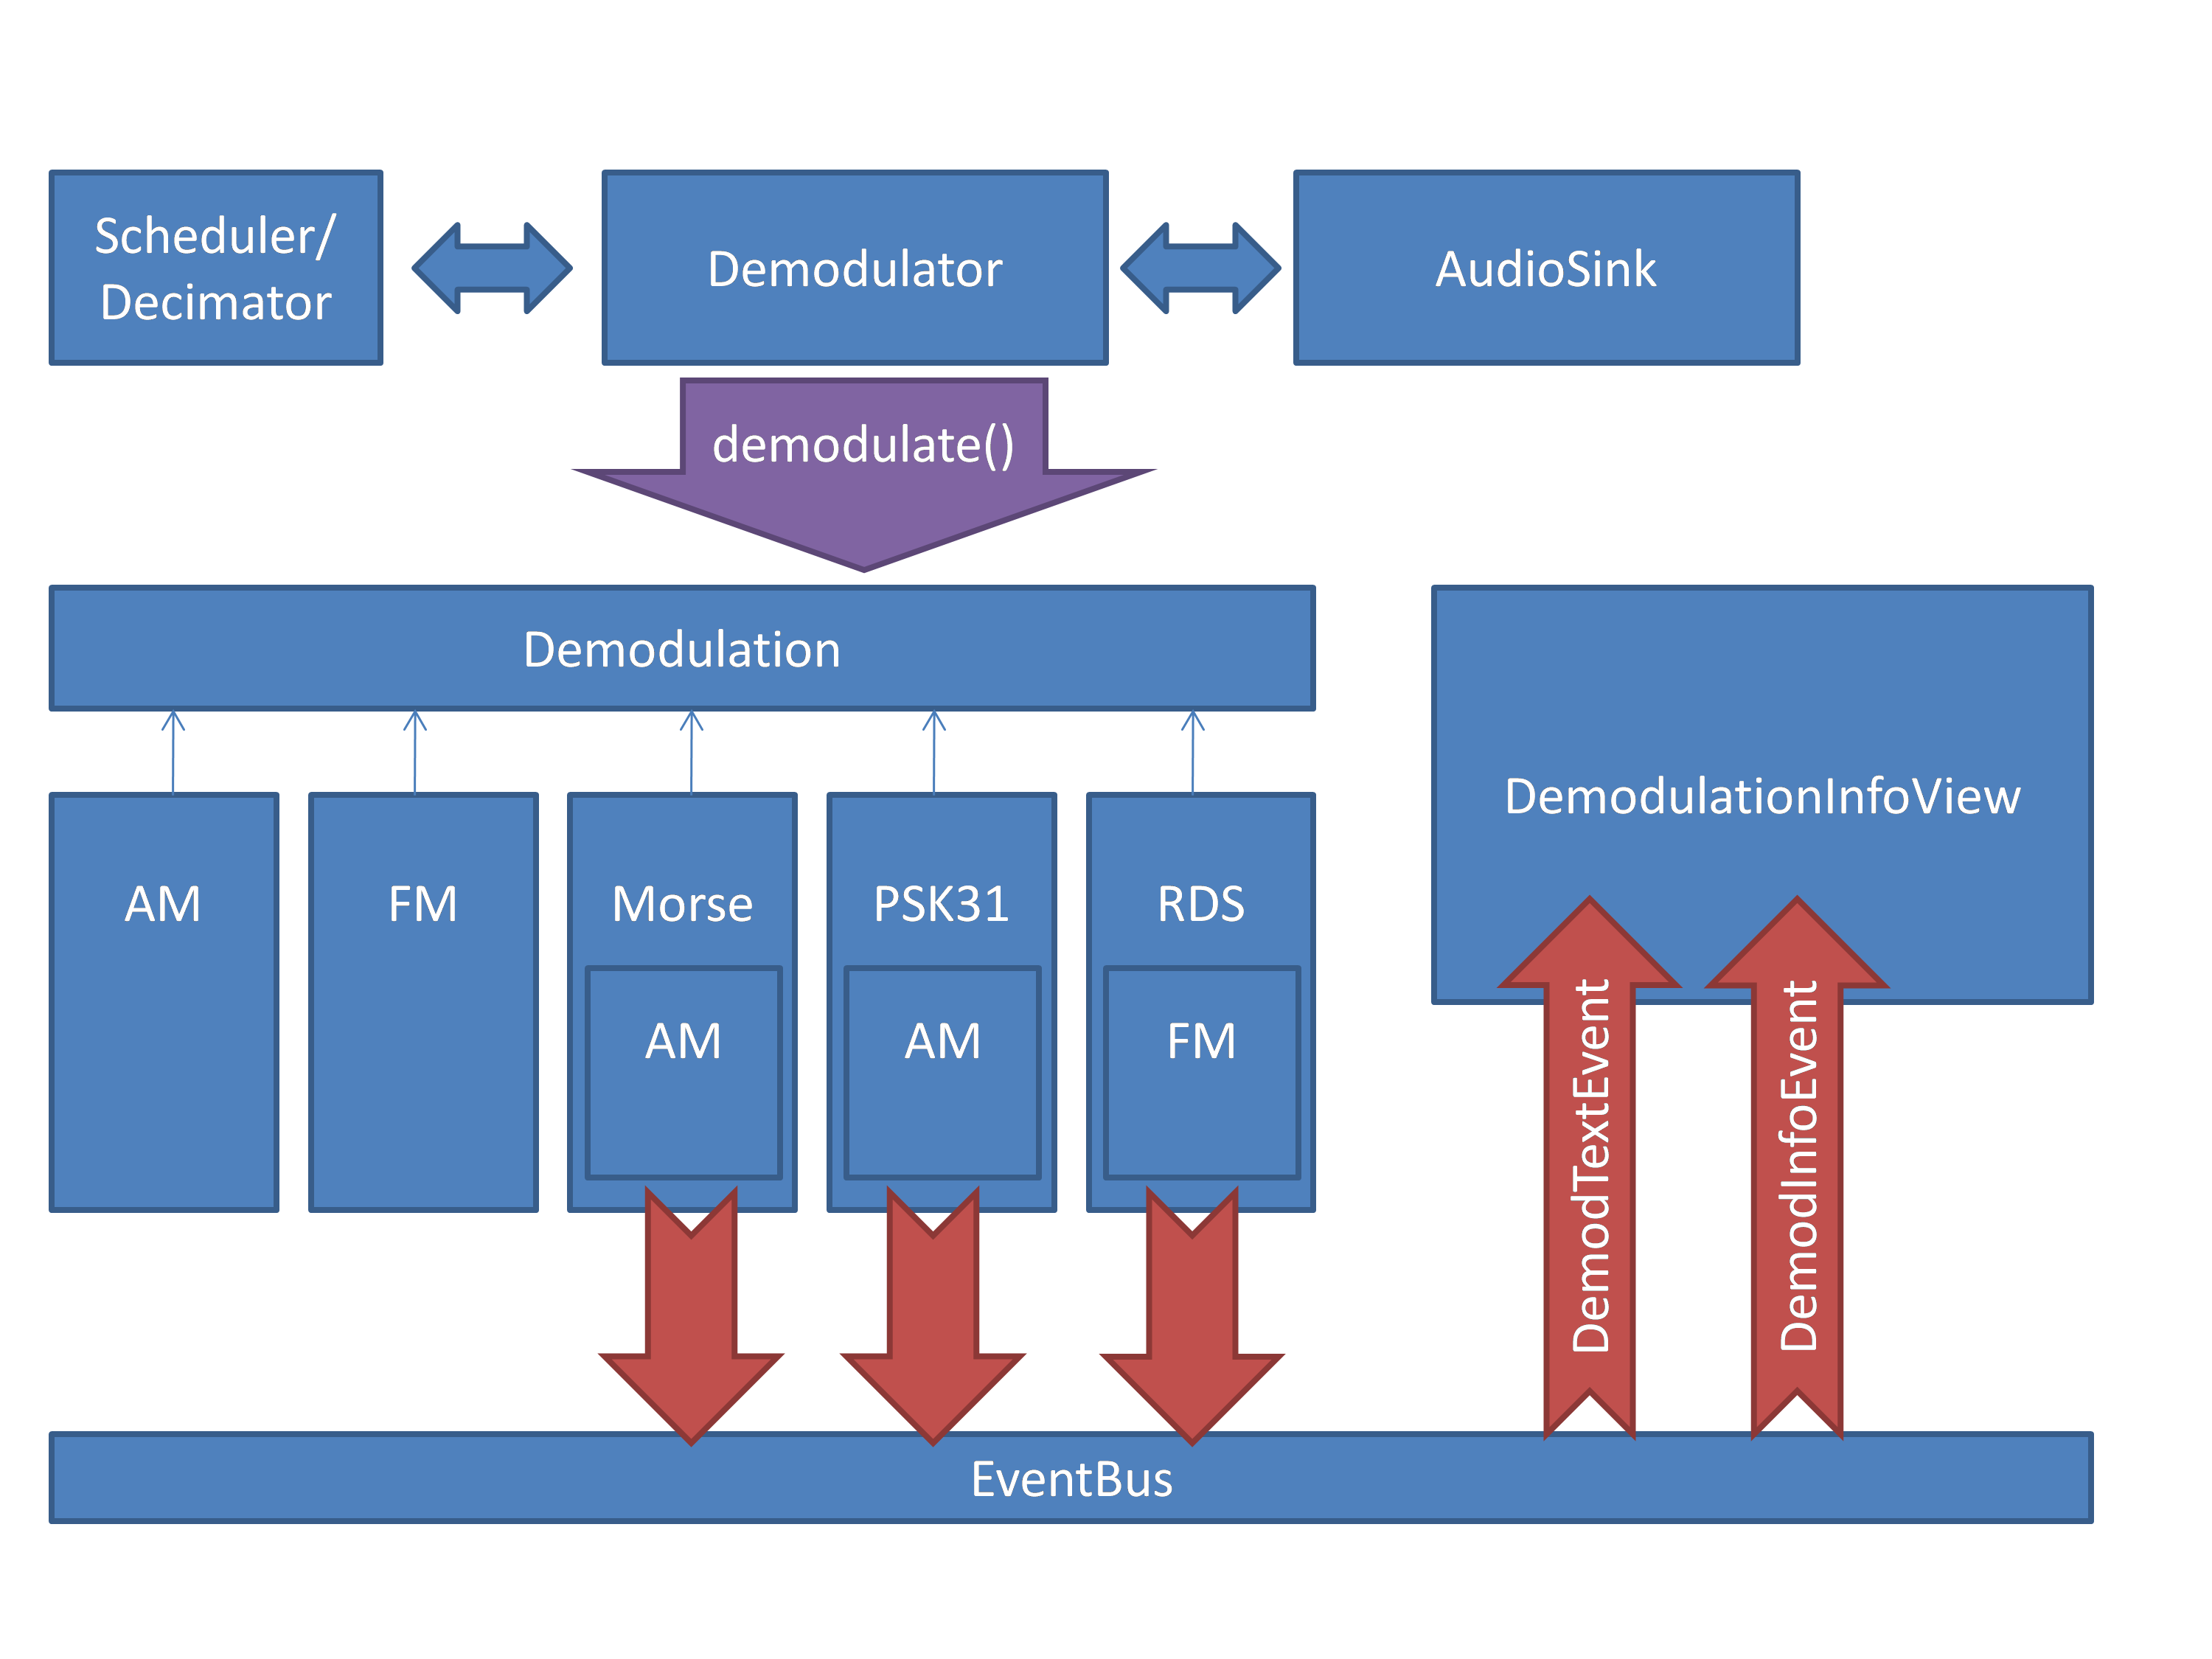
\includegraphics[width=1\linewidth]{gfx/demod_text_eventbus.png}
	\caption{Architecture of the extended demodulation logic and communication with the GUI}
	\label{fig:demod_text_eventbus}
\end{figure}

Two new classes \texttt{PSK31} and \texttt{RDS}, that inherit from
\texttt{Demodulation}, need to be implemented to represent the new demodulation 
mechanisms.

As \ac{PSK31} demodulation works on the envelope of the received signal
and \ac{AM} demodulation essentially performs envelope detection, \texttt{PSK31}
uses an instance of \texttt{AM} for envelope detection.

\ac{RDS} transmits metadata for \ac{FM} radio channels. It is therefore desirable for the 
\ac{RDS} demodulation mode to not only display this metadata, but to also play the 
\ac{FM}-modulated audio at the same time. The \texttt{RDS} class uses an
instance of \texttt{FM} for this purpose.

Like the existing architecture, the new architecture will use the EventBus
library to pass the demodulated text to the \ac{GUI}. The existing View
\texttt{MorseReceiveView} is refactored into a universal
\texttt{De\-mo\-du\-la\-tion\-In\-fo\-View} that displays the text output of any selected 
demodulator. Demodulators pass \texttt{DemodTextEvent}s and 
\texttt{DemodInfoEvent}s via the EventBus to the \texttt{De\-mo\-du\-la\-tion\-In\-fo\-View}, 
which contain demodulated text and further information (e.g. baud rates or raw 
dits and dahs) and are displayed in separate lines.

%************************************************
\chapter{Implementation}\label{ch:implementation} % $\mathbb{ZNR}$
%************************************************
%\glsresetall % Resets all acronyms to not used

\section{Radio Data System}

The \ac{RDS} signal is transmitted along with wide band \ac{FM}
radio signals to provide additional information about the
radio station and program.

Demodulation of the \ac{RDS} signal is first done in Octave in order to
evaluate the demodulation algorithm. The octave implementation
also helps by providing reference data of the different stages
of demodulation. 

\subsection{RDS modulation scheme}

\ac{RDS} uses \ac{BPSK} with Manchester encoding. The signal is
transmitted with an offset of 57 kHz relative to the center frequency
of the mono audio signal (baseband). The 19 kHz pilot tone of wideband \ac{FM}
can therefore be used to retrieve the \ac{RDS} carrier by multiplying
it with itself 3 times. The complete FM spectrum can be seen in
\autoref{fig:quad_demod_spectrum}.

After the \ac{RDS} baseband signal has been retrieved from the \ac{FM} signal
there are multiple ways of demodulating the \ac{BPSK} modulation. A sophisticated
approach tries to recover the phase synchronised \ac{RDS} carrier from the
signal by using e.g. a form of \ac{PLL} or Costas Loop. The symbols can then
be extracted by multiplying the carrier with the modulated signal and apply
a threshold operation to get bits.

A much simpler approach is to analyze the envelope of the signal and dectect
bits based on known shapes of ones and zeros in the waveform.
\autoref{fig:rds_envelope} shows the envelope and the pattern of symbols
which can be detected.

\begin{figure}
	\centering
	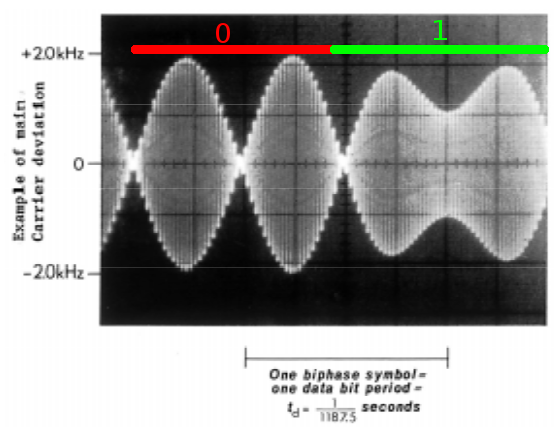
\includegraphics[width=1\linewidth]{gfx/rds/rds_waveform.png}
	\caption{RDS envelope waveform after Frequency demodulation. \cite{1999:iec62106}}
	\label{fig:rds_envelope}
\end{figure}



\subsection{RDS coding scheme}

RDS frames are called groups and each group consists of 4 blocks called
A, B, C and D. One block has a length of 16 bit plus a 10 bit checkword.
Block A always contains the \ac{PI} which identifies the radio station.
The content of the other blocks depends on the group type which is located
in block B (see \autoref{fig:rds_group0A}).

\begin{figure}
	\centering
	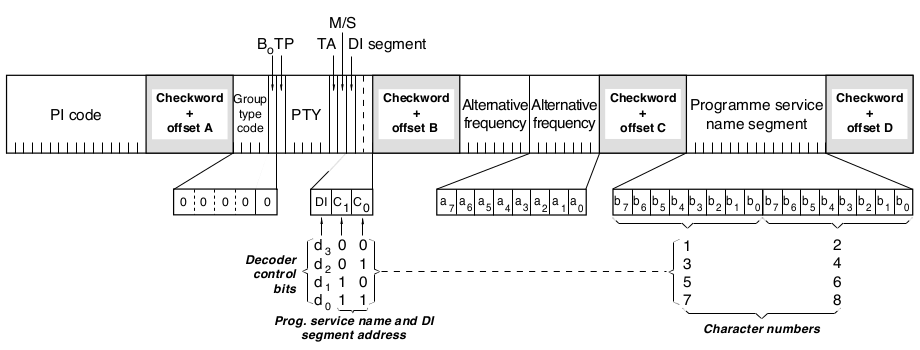
\includegraphics[width=1\linewidth]{gfx/rds/group0A.png}
	\caption{Coding scheme of RDS: group 0A. \cite{1999:iec62106}}
	\label{fig:rds_group0A}
\end{figure}

\begin{table}
	\begin{center}
		\begin{tabular}{ c c l }
		 Group Type & Group Version & Description \\\hline
		 0 & A & Basic tuning and switching information only \\
		 0 & B & Basic tuning and switching information only \\
		 1 & A & Programme Item Number and slow labelling codes\\
		 1 & B & Programme Item Number \\
		 2 & A & RadioText only \\
		 2 & B & RadioText only \\
		 3 & A & Applications Identification for ODA only \\
		 3 & B & Open Data Applications\\
		 4 & A & Clock-time and date only \\
		 4 & B & Open Data Applications\\
		 5 & A & Transparent Data Channels \\
		 5 & B & Transparent Data Channels \\
		 6 & A & In House applications or ODA \\
		 6 & B & In House applications or ODA \\
		 7 & A & Radio Paging or ODA \\
		 7 & B & Open Data Applications\\
		 8 & A & Traffic Message Channel or ODA \\
		 8 & B & Open Data Applications\\
		 9 & A & Emergency Warning System or ODA \\
		 9 & B & Open Data Applications\\
		10 & A & Programme Type Name\\
		10 & B & Open Data Applications\\
		11 & A & Open Data Applications\\
		11 & B & Open Data Applications\\
		12 & A & Open Data Applications\\
		12 & B & Open Data Applications\\
		13 & A & Enhanced Radio Paging or ODA\\
		13 & B & Open Data Applications\\
		14 & A & Enhanced Other Networks information only \\
		14 & B & Enhanced Other Networks information only \\
		15 & A & Defined in RBDS [15] only\\
		15 & B & Fast switching information only \\\hline
		\end{tabular}
		\caption{RDS Group Types}
		\label{tab:rds_groups}
	\end{center}
\end{table}

\autoref{tab:rds_groups} lists all group types and their descriptions.
The \ac{RDS} demodulation in AnSiAn only decodes types 0 and 2 because they contain
the basic information which is also often displayed on the radio
receiver.


\subsection{Evaluation in Octave}

Developing a signal processing application on Android has many drawbacks. One
issue is that it is very hard to debug the actuall signal processing components
because of the lack of proper tools to visualize and analyze the data that is
being processed. It is also not possible to do rapid prototyping without
sufficient signal processing libaries available. Therefore the \ac{RDS}
demodulator was first developed in Octave and afterwards ported to Android.

For development and testing it is better to work on recorded samples instead
of live captures. This makes tests reproducable and simplify the development
environment. The file was recorded using the record feature of RF Analyzer. It
can be imported to Octave by using the \emph{read\_cuchar\_binary()} script
provided by the GNU Radio project. After each step the produced output data
can be written back to an \emph{IQ} in order to use it in the Android application.
This way it is possible to develop each component of the demodulation process
separately and the output can be visualized on the developing machine.

The demodulation is done in the following steps:
\begin{enumerate}
	\item Downmixing the radio signal to baseband and filter it (see 
		\autoref{fig:rds_downmixing}).
	\item \ac{FM} demodulation (see \autoref{fig:quad_demod_spectrum}).
	\item Downmixing the \ac{RDS} signal to baseband and filter it
		(see \autoref{fig:rds_extraction} b and c).
	\item Take the absolute value of the signal to get the envelope
		that was shown above (see \autoref{fig:rds_waveform}).
	\item Find the beginning of a symbol by searching for a minimum in
		the waveform. From there find the end of the symbol with the
		same strategy. Now determine whether the symbol is a one or a
		zero according to the value of the minimum found in the middle
		of the sample compared to its peaks.
\end{enumerate}

\begin{figure}
\subfloat[Spectrum of the captured signal]{%
  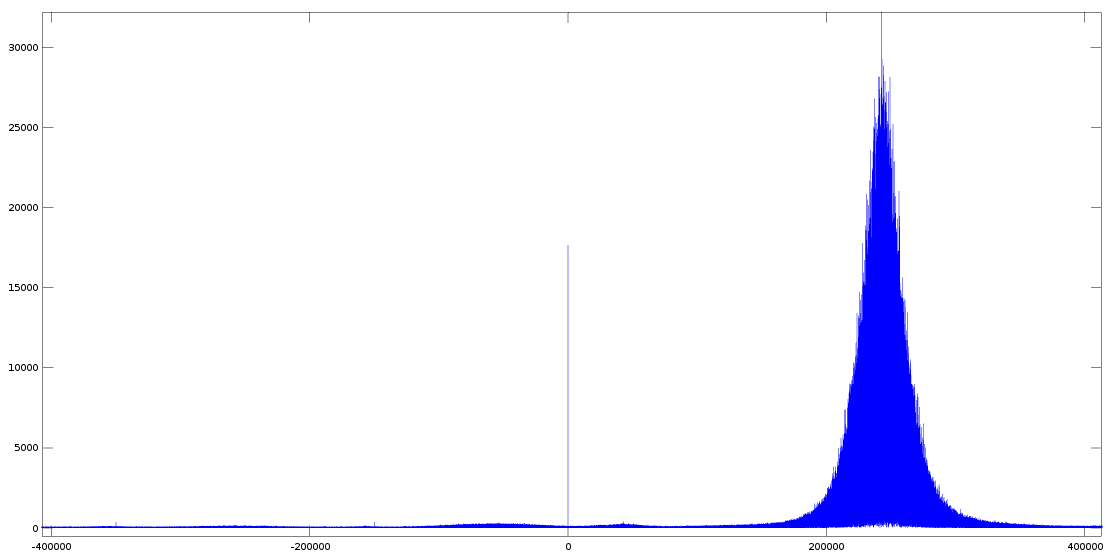
\includegraphics[clip,width=1\linewidth]{gfx/rds/raw_signal_spectrum.png}%
}

\subfloat[Spectrum after downmixing and filtering]{%
  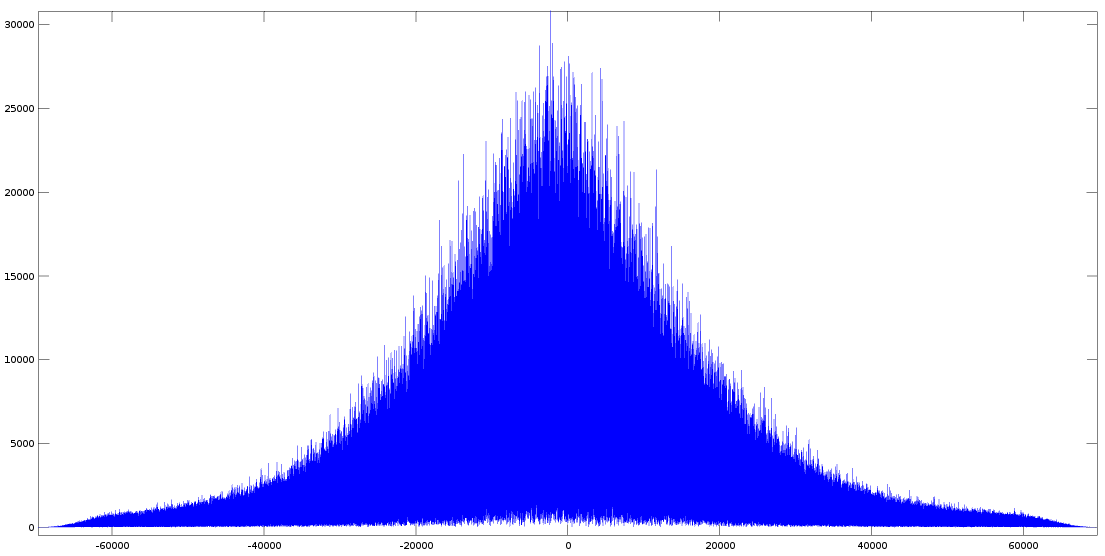
\includegraphics[clip,width=1\linewidth]{gfx/rds/fm_baseband_filtered_spectrum.png}%
}
\caption{FM Modulated Signal}
\label{fig:rds_downmixing}
\end{figure}


\begin{figure}
\subfloat[Signal spectrum after FM demodulation]{%
  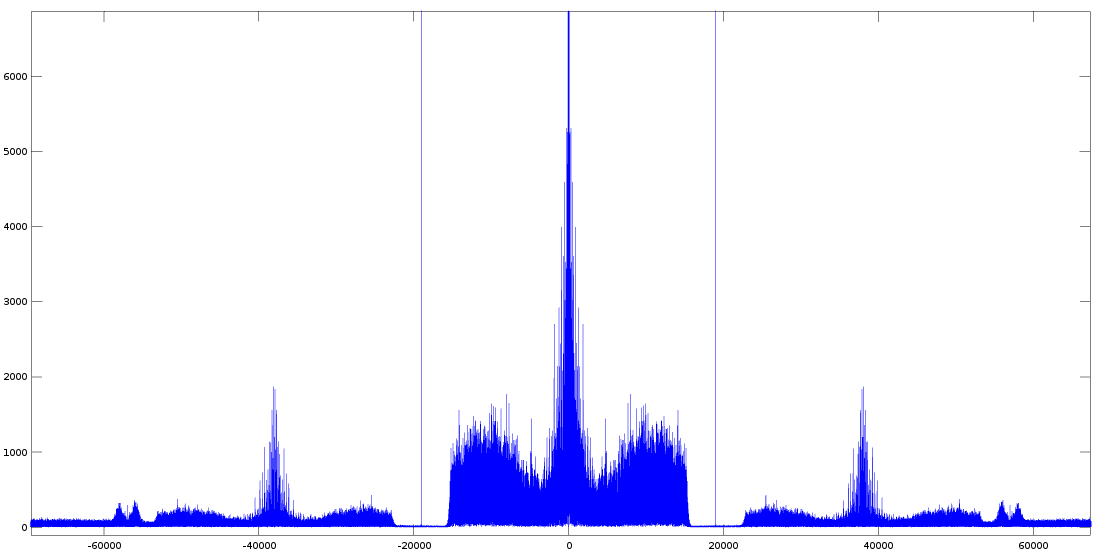
\includegraphics[clip,width=1\linewidth]{gfx/rds/quad_demod_spectrum.png}%
  \label{fig:quad_demod_spectrum}
}

\subfloat[RDS baseband spectrum after downmixing]{%
  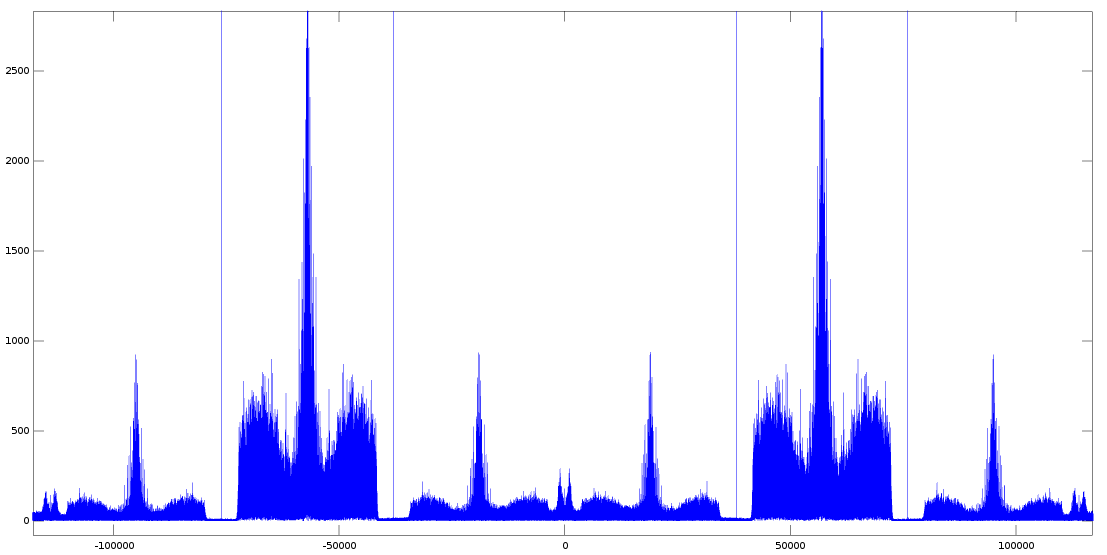
\includegraphics[clip,width=1\linewidth]{gfx/rds/rds_baseband_unfiltered_spectrum.png}%
}

\subfloat[RDS baseband spectrum after filtering]{%
  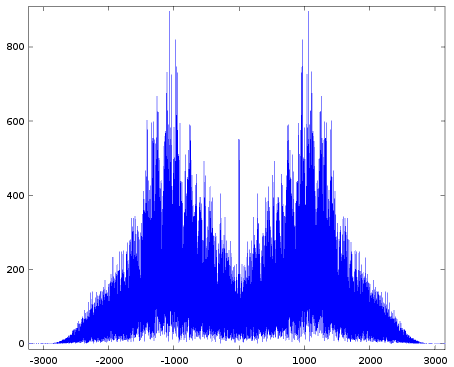
\includegraphics[clip,width=1\linewidth]{gfx/rds/rds_baseband_spectrum.png}%
}
\caption{Extracting the RDS signal from the FM signal}
\label{fig:rds_extraction}
\end{figure}

\begin{figure}
	\centering
	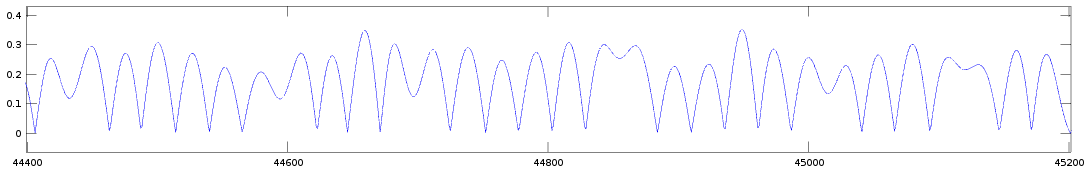
\includegraphics[width=1\linewidth]{gfx/rds/rds_magnitude_waveform.png}
	\caption{RDS waveform after take the absolute values}
	\label{fig:rds_waveform}
\end{figure}

The octave code used to execute the steps mentioned above is shown in the
listing below:

\begin{lstlisting}[label=lst:octave_rds, caption=Octave implementation of the RDS demodulator, language=none]
signal = read_cuchar_binary ("~/Downloads/2016-06-01-20-17-18_rtlsdr_100550000Hz_1000000Sps.iq" );
t = linspace(0, length(signal)/1000000, length(signal))';
carrier = e.^(2*pi*-245000*t*i);
down = carrier .* signal;
fl = fir1(300, 100000/1000000*2);
filtered = filter(fl, 1, down);
demod = quad_demod(filtered, 1);
t2 = linspace(0, length(demod)/1000000, length(demod));
rdscarrier = cos(2*pi*-57000*t2)';
rdsbase = demod(1:length(rdscarrier)) .* rdscarrier ;
frds = fir1(300, 2400/1000000*2);
rdsbase_filtered = filter(frds,1,rdsbase);
downsampled = decimate(rdsbase_filtered, 16).*80;
write_cuchar_binary (downsampled, "~/Downloads/rds_baseband_62500sps.iq");
bits = rds_bpsk_demodulate(downsampled, 62500);
rds_decode(bits)
\end{lstlisting}

The \emph{quad\_demod()} function does the quadrature demodulation
(FM demodulation). The \emph{rds\_bpsk\_demodulate()} function is shown
in the following listing:

\begin{lstlisting}[label=lst:octave_rds_bpsk, caption=Octave implementation of the BPSK demodulation, language=none]
function demod = rds_bpsk_demodulate(signal, fs)
  samples_per_symbol = fs/1187.5
  samples_per_symbol = ceil(samples_per_symbol)
  envelope = abs(signal);
  
  % Find the first minimum
  [minimum, idx1] = min(envelope(1:samples_per_symbol))
  
  bits = [];
  while (idx1 + samples_per_symbol*2 < length(envelope))
    % find end of symbol idx2 (minimum near idx1 + samples_per_symbol)
    from = round(idx1+samples_per_symbol*0.75);
    to   = round(idx1+samples_per_symbol*1.25);
    [minimum, idx2] = min(envelope(from:to));
    idx2 = idx2 + from;
    
    % calc mean of all samples between idx1 and idx2 and calc threshold = mean/2
    m = mean(envelope(idx1:idx2));
    threshold = m/2;
    
    % get minimum sample in the middle between idx1 and idx2 ...
    span = idx2 - idx1;
    from = round((idx1+idx2)*0.5 - 0.25*span);
    to   = round((idx1+idx2)*0.5 + 0.25*span);
    [minimum, idxmiddle] = min(envelope(from:to));
    idxmiddle = idxmiddle + from;
    
    % Check whether we have the correct timing. It might be, that idx2 is
    % actually in the middle of a symbol than at its end.
    if (envelope(idx2) > threshold)
      % In this case we find the minimum between idx1 and idx2 and set it
      % as idx1 for the next round:
      %printf("WARNING: Wrong timing. thres=%f < envelope(idx2=%d)=%f\n",threshold,idx2,envelope(idx2));
      idx1 = idxmiddle;
      continue;
    endif
    
    % ... and check it against the threshold
    s = envelope(idxmiddle);
    if (s > threshold)
      bits = [bits 1];
    else
      bits = [bits 0];
    endif
    
    % idx1 = idx2 and continue with the next symbol..
    idx1 = idx2;
    
  endwhile
  demod = bits;
\end{lstlisting}


\subsection{Android Implementation}

For the Android implementation two classes are added to the AnSiAn codebase:
\begin{itemize}
	\item BPSK: This class handles the \ac{BPSK} demodulation and can be
		reused by other demodulators using the \ac{BPSK} modulation scheme
		(e.g. PSK31).
	\item RDS: This class integrates in the existing FM class for frequency
		demodulation. It handles the decoding and processing of \ac{RDS}
		groups. 
\end{itemize}

A screenshot of the application demodulating the \ac{RDS} signal of the
\emph{Antenne Frankfurt} station is shown in \autoref{fig:rds_android_screenshot}.

\begin{figure}
	\centering
	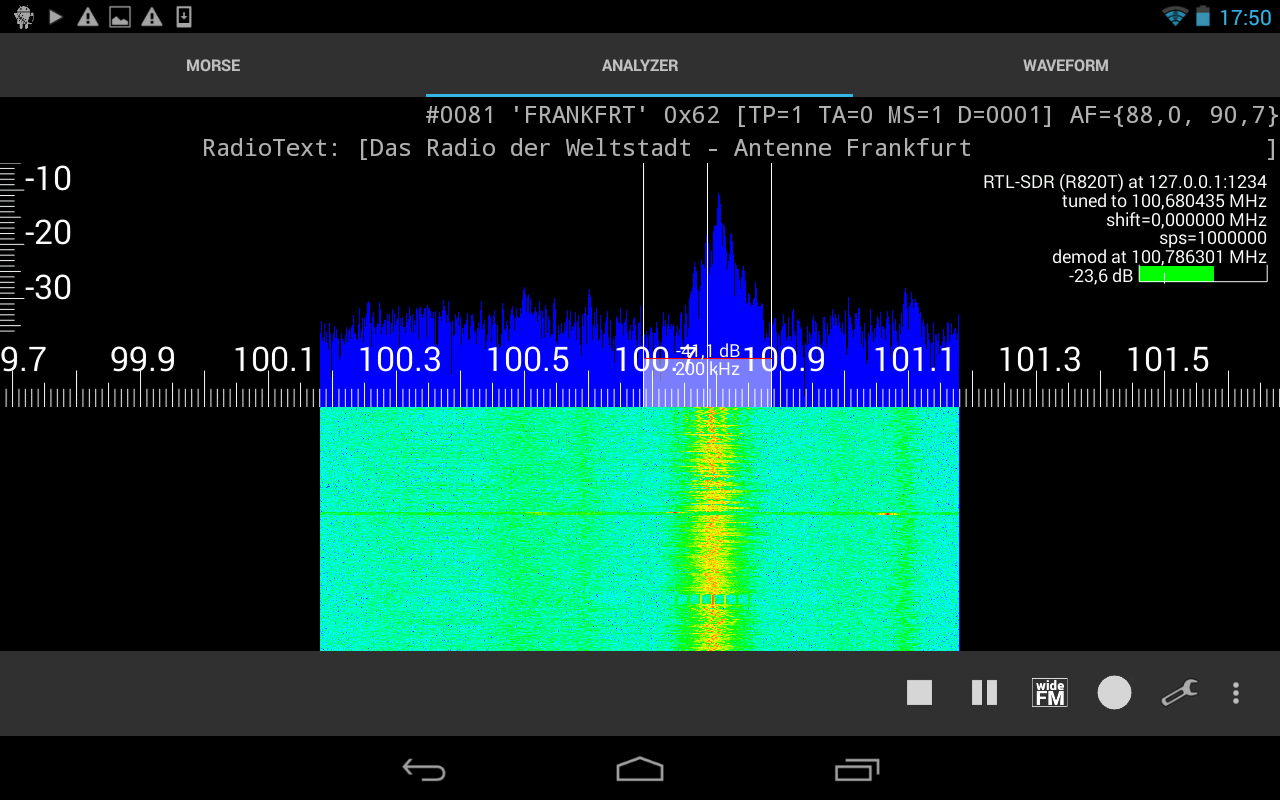
\includegraphics[width=1\linewidth]{gfx/rds/android_screenshot.png}
	\caption{Screenshot of the RDS demodulator on a Nexus 7}
	\label{fig:rds_android_screenshot}
\end{figure}


%************************************************
%\chapter{Evaluation}\label{ch:evaluation} % $\mathbb{ZNR}$
%************************************************
%\glsresetall % Resets all acronyms to not used


%%************************************************
\chapter{Discussion}\label{ch:Discussion} % $\mathbb{ZNR}$
%************************************************
\glsresetall % Resets all acronyms to not used

\lipsum[6]

%************************************************
\chapter{Conclusions}\label{ch:Conclusions} % $\mathbb{ZNR}$
%************************************************
\glsresetall % Resets all acronyms to not used

\lipsum[7]

% ********************************************************************
% Backmatter
%*******************************************************
\appendix
%\cleardoublepage
%\part{Appendix}
%%********************************************************************
% Appendix
%*******************************************************
% If problems with the headers: get headings in appendix etc. right
%\markboth{\spacedlowsmallcaps{Appendix}}{\spacedlowsmallcaps{Appendix}}
\chapter{Appendix}\label{ch:Appendix}
\glsresetall % Resets all acronyms to not used

\lipsum[8]

%********************************************************************
% Other Stuff in the Back
%*******************************************************
% not yet. ADD BACK LATER!
%\cleardoublepage%********************************************************************
% Bibliography
%*******************************************************
% work-around to have small caps also here in the headline
\manualmark
\markboth{\spacedlowsmallcaps{\bibname}}{\spacedlowsmallcaps{\bibname}} % work-around to have small caps also
%\phantomsection 
\refstepcounter{dummy}
\addtocontents{toc}{\protect\vspace{\beforebibskip}} % to have the bib a bit from the rest in the toc
\addcontentsline{toc}{chapter}{\tocEntry{\bibname}}
\label{app:bibliography}
\printbibliography

\cleardoublepage% ******************************************************* Declaration
% *******************************************************
\refstepcounter{dummy}
\selectlanguage{ngerman}
\pdfbookmark[0]{Erklärung}{erklaerung} \chapter*{Erklärung}
\thispagestyle{empty}
Hiermit versichere ich gemäß der Allgemeinen Prü"-fungs"-be"-stim"-mun"-gen der
Technischen Universität Darmstadt (APB) §\,23\,(7), die vorliegende Masterarbeit
ohne Hilfe Dritter und nur mit den angegebenen Quellen und Hilfsmitteln
angefertigt zu haben. Alle Stellen, die aus den Quellen entnommen wurden, sind
als solche kenntlich gemacht worden. Diese Arbeit hat in gleicher oder ähnlicher
Form noch keiner Prüfungsbehörde vorgelegen.
\bigskip
 
\noindent\textit{\myLocation, \myTime}

\smallskip

\begin{flushright}
    \begin{tabular}{m{5cm}}
        \\ \hline
        \centering\myName \\
    \end{tabular}
\end{flushright}

% ********************************************************************
% Game Over: Restore, Restart, or Quit?
%*******************************************************
\end{document}
% ********************************************************************
